\chapter{Investigation of reflection and refraction at media interface}\label{lec:lec31}
Here we will investigate how much energy is reflected and how much is transmitted at the media interface. We are still considering lossless media as in the previous lectures for which conductivity, $ \sigma = 0$, but the two media could have different permeability and permittivity.

\begin{figure}[h]
\centering
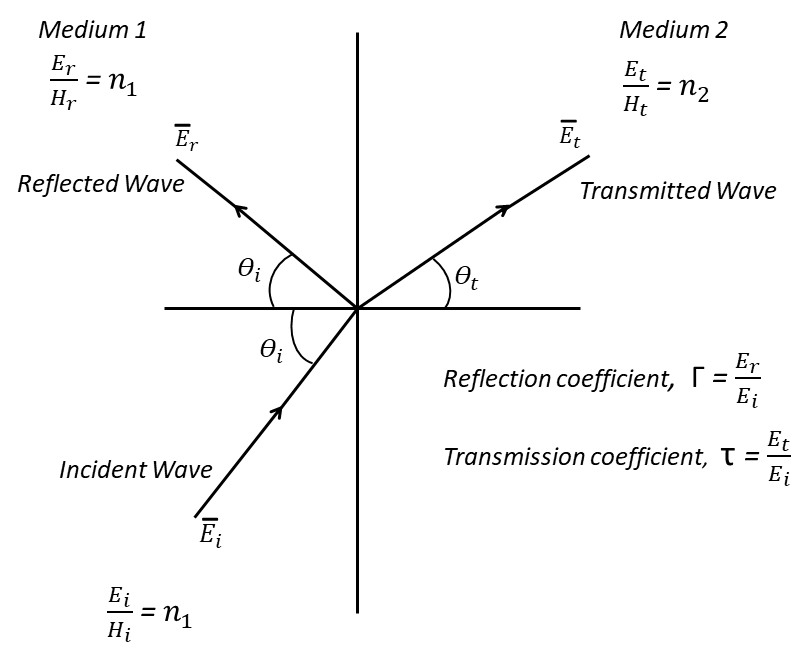
\includegraphics[width=1\linewidth]{./graphics/reflection_refraction1}
\caption{Reflection and refraction at dielectric media interface}
\label{fg:11}
\end{figure}

So as we have seen, we have a media interface with different medium properties on either side of the interface and at this point, we want to determine two important quantities which are the \textbf{Reflection coefficient}(the ratio of the amplitude of the reflected wave to the amplitude of the incidence wave) and the \textbf{Transmission coefficient}(the ratio of the amplitude of the transmitted wave to the amplitude of the incident wave). We will define these quantities for the electric fields only because as we know since the wave nature still remains a plane wave, we can always determine the magnetic fields of the wave(ie incident, reflected and transmitted wave) corresponding to the electric fields when required.
So we basically write down the electric and magnetic fields for the three waves(ie incident, reflected and transmitted waves) for the two media and then apply boundary conditions at the interface and by doing some algebra, we get $\frac{E_{r}}{E_{i}}$ and $\frac{E_{t}}{E_{i}}$ for the reflection coefficient and transmission coefficient respectively. However the electric field $\bar{E}$ is a vector quantity so when the wave is incident on the dielectric media interface, the electric field vector in general will make an arbitrary angle with respect to the plane of incidence. This makes the analysis complicated. So to avoid this, generally we split the problem into two. We take the two components of the electric field where one component is perpendicular to the plane of incidence and the other lie in the plane of incidence.
So essentially, we now have two cases for which we can determine the reflection and transmission coefficients.

Thus, the problem of reflection and refraction at the dielectric media interface has been decomposed into two which are;

\begin{enumerate}[(i)]
\item When the electric field is perpendicular to the plane of incidence which we call \emph{Perpendicular polarization}.
\item When the electric field is parallel or lies in the plane of incidence which we call \emph{Parallel polarization}.
\end{enumerate}

Now we will find out the reflection coefficient $\Gamma$ and the transmission coefficient $\tau$ for each of the two cases.

\section{Perpendicular polarization} 
From the diagram below the wave is incident at an angle $\theta_{i}$ to the normal. The wave vector lies on the plane of the paper or the plane of incidence. For perpendicular polarization, the electric field $\bar{E}$ must either be coming out of the paper in the positive y direction or going into the paper in the negative y direction.
\begin{figure}[h]
\centering
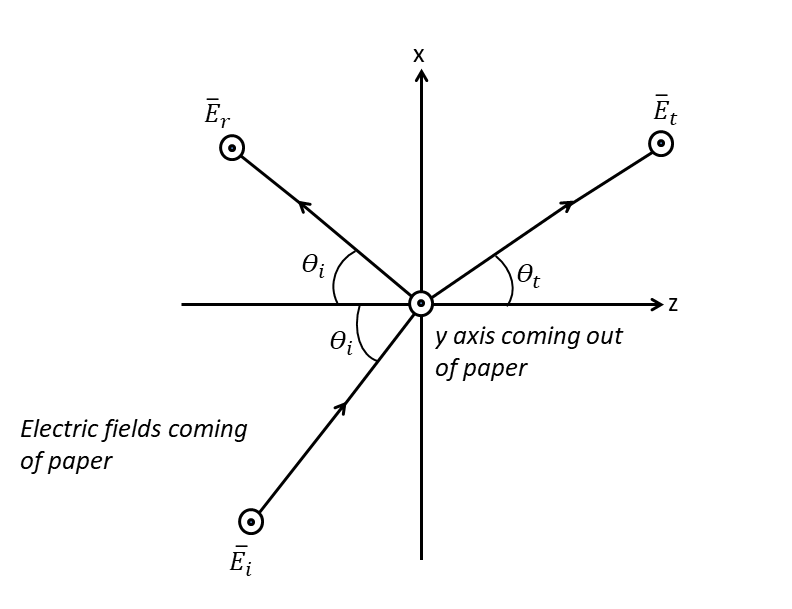
\includegraphics[width=1\linewidth]{./graphics/perpendicular_polarization1}
\caption{Perpendicular polarization}
\label{fig:12}
\end{figure}

To satisfy the boundary condition, at the interface, the tangential component of an electric field across the boundary should be continuous. Thus, if $\bar{E}_{i}$ is y oriented, then both  $\bar{E}_{r}$ and  $\bar{E}_{t}$ must be y oriented.
\begin{figure}[h]
\centering
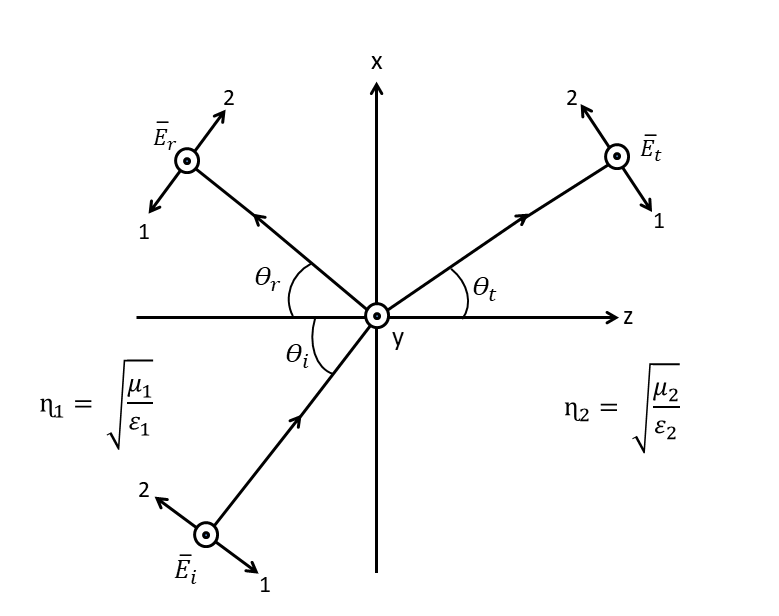
\includegraphics[scale=0.44]{./graphics/perpendicular_polarization2}
\caption{}
\label{fig:13}
\end{figure}

$\bar{E}_{i}$, $\bar{E}_{r}$ and  $\bar{E}_{t}$ may not all necessarily be in the positive y direction but let's say they are in the positive y direction so  $\bar{E}_{i}$,  $\bar{E}_{r}$ and  $\bar{E}_{t}$ are all assumed to be coming out of the plane of the paper. Now we have to write down the corresponding magnetic fields for which we use the pointing Vector argument. We must choose the direction of the magnetic fields $\bar{H}$ such that the pointing vector will be in the direction of the wave propagation or wave vector(this can be easily done using the right-hand rule). Since $\bar{E}$ for all 3 electric fields is perpendicular to the plane of the paper, then the $\bar{H}$ field vector for all 3 must lie in the plane of the paper or plane of incidence. They can go in either direction 1 or 2 as shown in the figure~\ref{fig:13} depending on whether the electric field vector $\bar{E}$ is coming out or going into the plane of incidence. This will be decided by the pointing vector of  $\bar{E} \times \bar{H}$ giving the wave direction. Since we are dealing with transverse electromagnetic waves $\frac{E}{H} = \eta$, so that $\frac{E_{i}}{H_{i}} = \eta_{1}$, $\frac{E_{r}}{H_{r}} = \eta_{1}$ and  $\frac{E_{t}}{H_{t}} = \eta_{2}$.

Again we decompose the magnetic fields into their various components along the x and z directions. E is already perpendicular to the plane of the paper as shown in figure~\ref{fig:14}.
\begin{figure}[h]
\centering
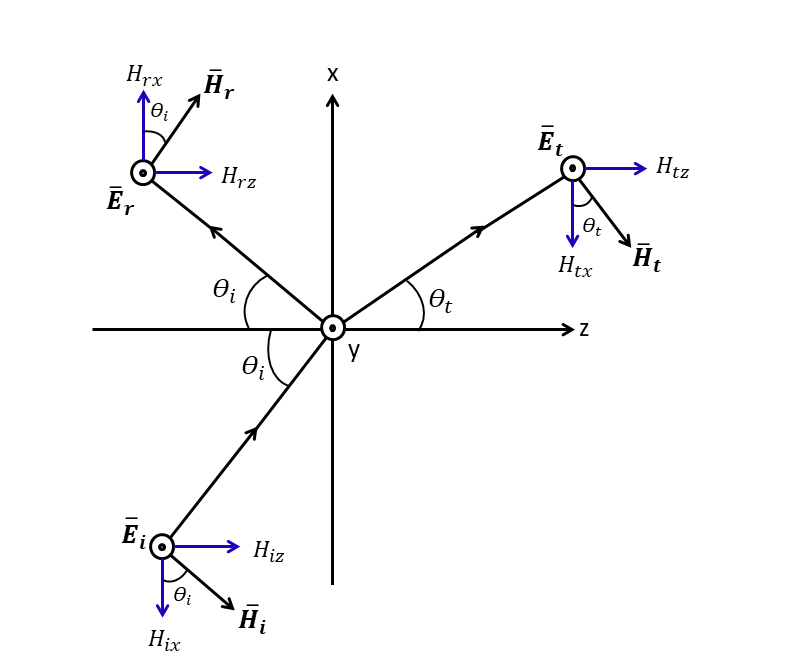
\includegraphics[width=1.2\linewidth]{./graphics/perpendicular_polarization3}
\caption{}
\label{fig:14}
\end{figure}

From figure~\ref{fig:14} the expressions for the electric fields can be evaluated as;
\begin{align*}
\bar{E_{i}} = E_{1} e^{-j\beta_{1} (x sin\theta_{i} + z cos\theta_{i})} \hat{y}\\
\bar{E_{r}} = E_{r} e^{-j\beta_{1} (x sin\theta_{i} - z cos\theta_{i})} \hat{y}\\
\bar{E_{t}} = E_{t} e^{-j\beta_{2} (x sin\theta_{t} + z cos\theta_{t})} \hat{y}
\end{align*}

To satisfy the boundary conditions, since all 3 fields are tangential to the boundary at $z=0$, then the sum of $E_i$ and $E_r$ should be equal to $E_{t}$ as the tangential component of $\bar{E}$ should be continuous at $z=0$ i.e at the boundary or media interface.
Hence,
\begin{align*}
E_{i} e^{-j \beta_{i} x sin\theta_{i}} + E_{r} e^{-j \beta_{1} x sin\theta_{i}} = E_{t} e^{-j \beta_{2} x sin\theta_{t}}
\end{align*}
We recall from snells law that $\beta_{1} sin\theta_{i} = \beta_{1} sin\theta_{i} = \beta_{2} sin\theta_{t}$. Thus the phase function is the same for all the 3 waves, hence the phase term is common.

This implies that $ E_{i} + E_{r} = E_{t}$. This relationship is true whether for normal or tangential components since this phase function is always the same for the three waves. So the component we take for electric or magnetic field is immaterial, as the phase function remains the same so that the boundary condition can be applied only to the amplitude terms. 
\begin{equation}
E_{i} + E_{r} = E_{t}
\label{eqn:eqn31_1}
\end{equation}
Since we are talking about dielectric media, there are no surface currents, so we can also apply the continuity of the tangential component for the magnetic fields. Recall that the tangential component continuity cannot be assumed if there is the possibility of surface current. As we have seen surface current is for conductors. So with a dielectric boundary like this, there are no surface currents, thus, the continuity of the tangential component of the magnetic fields can be applied so that; 
\begin{equation*}
H_{ix} - H_{rx} = H_{tx}
\end{equation*}
\begin{equation*}
H_{i} cos\theta_{i} - H_{r} cos\theta_{i} = H_{t} cos\theta_{t}
\end{equation*}
So, substituting for $H_{i}$, $H_{r}$ and $H_{t}$,
\begin{equation}
\frac{E_{i}}{\eta_{1}} cos\theta_{i} - \frac{E_{r}}{\eta_{1}} cos\theta_{i} = \frac{E_{t}}{\eta_{2}} cos\theta_{t}
\label{eqn:eqn31_2}
\end{equation}
Recall that we are interested in finding out the quantities; \emph{reflection coefficient}, $\Gamma = \frac{E_{r}}{E_{i}}$ and \emph{transmission coefficient}, $ \tau = \frac{E_{t}}{E_{i}}$, and using equation~\ref{eqn:electric} and equation~\ref{eqn:eqn31_2}, we can determine the \emph{reflection} and \emph{transmission coefficient}.

\begin{enumerate}[(i)]
\item REFLECTION COEFFICIENT FOR PERPENDICULAR POLARIZATION
$$\Gamma_{\bot} = \frac{\eta_{2} cos\theta_{i} - \eta_{1} cos\theta_{t}}{\eta_{2} cos\theta_{i} + \eta_{1} cos\theta_{t}}$$
\item TRANSMISSION COEFFICIENT FOR PERPENDICULAR POLARIZATION
$$\tau_{\bot} = \frac{2 \eta_{2} cos\theta_{i}}{\eta_{2} cos\theta_{i} + \eta_{1} cos\theta_{t}}$$
\end{enumerate}
The above expressions are proven below;

Dividing equation~\ref{eqn:eqn31_1} and equation~\ref{eqn:eqn31_2} by $E_{i}$ , we have
\begin{equation*}
\frac{E_{i}}{E_{i}} + \frac{E_{r}}{E_{i}} = \frac{E_{t}}{E_{i}}
\end{equation*}
or
\begin{equation*}
1 + \Gamma = \tau
\end{equation*}

\begin{equation*}
\frac{E_{i}}{E_{i}\eta_{1}}cos\theta_{i} - \frac{E_{r}}{E_{i}\eta_{1}}cos\theta_{i} = \frac{E_{t}}{E_{i}\eta_{2}}cos\theta_{t}
\end{equation*}

\begin{equation*}
\frac{1}{\eta_{1}}cos\theta_{i} - \frac{\Gamma}{\eta_{1}}cos\theta_{i} = \frac{\tau}{\eta_{2}}cos\theta_{t}
\end{equation*}
but $1 + \Gamma = \tau$
\begin{dmath*}
\frac{1}{\eta_{1}}cos\theta_{i} - \frac{\Gamma}{\eta_{1}}cos\theta_{i} = \frac{1+\Gamma}{\eta_{2}}cos\theta_{t} = \frac{1}{\eta_{2}}cos\theta_{t} + \frac{\Gamma}{\eta_{2}}cos\theta_{t}
\end{dmath*}
\begin{equation*}
\frac{1}{\eta_{1}}\cos\theta_{i} - \frac{1}{\eta_{2}}cos\theta_{t} 	= \Gamma( \frac{1}{\eta_{2}}cos\theta_{t} + \frac{1}{\eta_{1}}cos\theta_{i})
\end{equation*}
$$\eta_{2}cos\theta_{i} - \eta_{1}cos\theta_{t} = \Gamma(\eta_{1}cos\theta_{t} + \eta_{2}cos\theta_{i})$$
So
$$\Gamma = \frac{\eta_{2}cos\theta_{i} - \eta_{1}cos\theta_{t}}{\eta_{2}cos\theta_{i} + \eta_{1}cos\theta_{t}}$$
and
\begin{dmath*}
\tau = 1 + \Gamma = 1 + \frac{\eta_{2}\cos\theta_{i} - \eta_{1}\cos\theta_{t}}{\eta_{2}\cos\theta_{i} + \eta_{1}\cos\theta_{t}}
= \frac{\eta_{2}\cos\theta_{i} + \eta_{1}cos\theta_{t} + \eta_{2}cos\theta_{i} - \eta_{1}cos\theta_{t}}{\eta_{2}\cos\theta_{i} + \eta_{1}\cos\theta_{t}} = \frac{2 \eta_{2}\cos\theta_{i}}{\eta_{2}\cos\theta_{i} + \eta_{1}\cos\theta_{t}}
\end{dmath*}
hence for perpendicular polarization,
\begin{dmath}
\Gamma_{\perp} = \frac{\eta_{2}cos\theta_{i} - \eta_{1}cos\theta_{t}}{\eta_{2}cos\theta_{i} + \eta_{1}cos\theta_{t}}
\label{eqn:eqn31_3}
\end{dmath}
\begin{dmath}
\tau_{\perp} = \frac{2 \eta_{2}cos\theta_{i}}{\eta_{2}cos\theta_{i} + \eta_{1}cos\theta_{t}}
\label{eqn:eqn31_4}
\end{dmath}


So once $E_{r}$ and $E_{t}$ are obtained, then we have the phase function. We can find out the wave at any location and at any point in space in medium 1 and in medium 2. In medium  1, we have a superposition of the wave $E_{r}$ and $E_{i}$.

In medium 2 we have only $E_{t}$. Two things are observed from the expressions for the reflection and transmission coefficient.
\begin{enumerate}[(i)]
\item The reflection coefficient is always less than or equal to 1 that is, $|\Gamma_{\bot}| \leq 1$ but $\tau_{\bot}$ could be less than 1 or greater than 1. The pointing vector is proportional  to $|\bar{E}|^{2}$. So if $|\Gamma_{\bot}|< 1$, that means the pointing vector magnitude for the reflected wave is always less than 1 and the power density of the reflected wave is always going to be less than that of the incident wave.
\item $\tau$ on the other hand could be greater than or less than 1.  $\tau_{\bot} > 1$ means that the electric field in medium 2 will be larger than that of the incident electric field. This does not mean that the pointing vector in medium 2 (representing power density) is more than that of medium 1. Although the electric field is larger in medium 2, from the intrinsic impedance $\eta=\sqrt{\frac{\mu}{\epsilon}}$ and $\frac{E}{\eta} =H$, the magnetic field reduces correspondingly thereby making the pointing vector of the transmitted wave always less than that of the incident wave. Moreover, the law of conservation of energy must hold so the power density incident must be equal to the power density transmitted plus the power density reflected.
\end{enumerate}
It's important to also note that, when a wave is reflected from the boundary, there may be a phase reversal for the wave or there may be no phase reversal for the wave. The incident wave and transmitted wave are always in phase as $\tau$ is always positive but $\Gamma_{\perp}$ can be positive or negative hence, $E_{i}$ and $E_{r}$ can be in phase ($\Gamma_{\perp}$ positive) or out of phase i.e $\Gamma_{\perp}$ is negative. This means that if $E_{i}$ is in the positive y direction(ie coming out of the plane of the paper), then $E_{t}$ will always be coming out of the paper, but the reflected wave $E_{r}$ may be coming out of the paper(if $\Gamma_{\perp}$ is positive) or going in(if $\Gamma_{\perp}$ is negative).

These are the important conclusions that we can draw for the perpendicularly polarized wave.

\section{Parallel polarization}
With $\bar{H}$ coming out of the plane of the paper, $\bar{E}$ must lie on the plane of the paper or the plane of incidence. As we saw in the previous case, since the phase function is the same for the three waves and there is continuity of the tangential component of the magnetic fields, we get
\begin{equation*}
H_{i} + H_{r} = H_{t}
\end{equation*}
or
\begin{figure}[h]
\centering
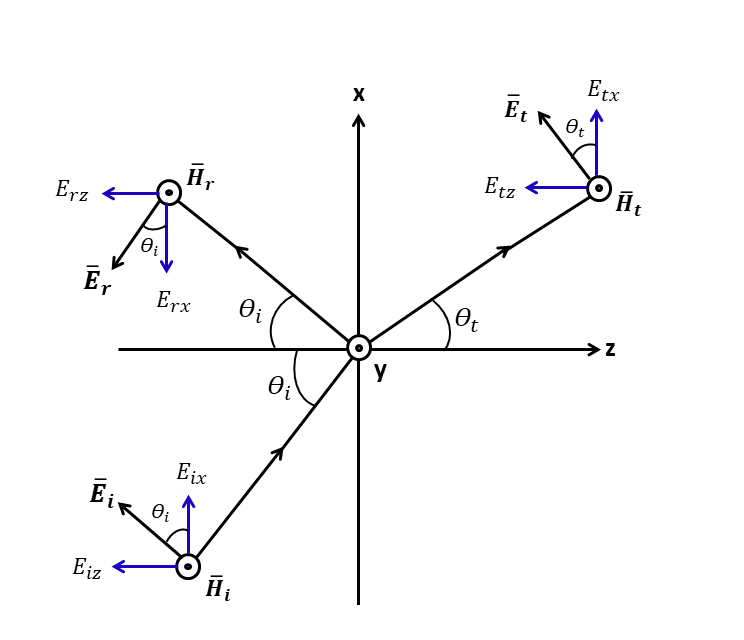
\includegraphics[width=1.2\linewidth]{./graphics/parallel_polarization1}
\caption{}
\label{fig:15}
\end{figure}
\begin{equation}
\frac{E_{i}}{\eta_{1}} + \frac{E_{r}}{\eta_{1}} = \frac{E_{t}}{\eta_{2}}
\label{eqn:eqn31_5}
\end{equation}
And for the electric field,
\begin{equation*}
E_{ix} - E_{rx} = E_{tx}
\end{equation*}
\begin{equation}
E_{i} cos\theta_{i} - E_{r} cos\theta_{i} = E_{t} cos\theta_{t}
\label{eqn:eqn31_6}
\end{equation}
dividing equation~\ref{eqn:eqn31_5} by $E_{i}$ we have;
\begin{equation}
\frac{1}{\eta_{1}} + \frac{\Gamma}{\eta_{1}} = \frac{\tau}{\eta_{2}}
\label{eqn:eqn31_7}
\end{equation}
similarly dividing  equation~\ref{eqn:eqn31_6} by $E_{i}$ we have;
\begin{equation}
cos\theta_{i} - \Gamma cos\theta_{i} = \tau cos\theta_{t}
\end{equation}
\begin{equation*}
\tau = \frac{1}{cos\theta_{t}} (cos\theta_{i} - \Gamma cos\theta_{i})
\end{equation*}
substituting into equation~\ref{eqn:eqn31_7} we get;
\begin{align*}
\frac{1}{\eta_{1}} + \frac{\Gamma}{\eta_{1}} &= \frac{1}{\eta_{2}} \frac{1}{\cos\theta_{t}} (\cos\theta_{i} - \Gamma \cos\theta_{i})\\
\frac{1}{\eta_{1}} + \frac{\Gamma}{\eta_{1}} &= \frac{\cos \theta_{i}}{\eta_{2}\cos \theta_{t}} - \frac{\Gamma \cos\theta_{i}}{\eta_{2} \cos\theta_{t}}\\
\Gamma \left(\frac{1}{\eta_{1}} + \frac{\cos\theta_{i}}{\eta_{2} cos\theta_{t}}\right) &= \frac{cos\theta_{i}}{\eta_{2} \cos\theta_{t}} - \frac{1}{\eta_{1}}\\
\Gamma \left(\frac{\eta_{2} \cos\theta_{t} + \eta_{i} \cos\theta_{i}}{\eta_{1} \eta_{2} \cos\theta_{t}}\right) &= \frac{\eta_{1} cos\theta_{i} - \eta_{2} \cos\theta_{t}}{\eta_{1} \eta_{2} \cos\theta_{t}}\\
\Gamma &= \frac{\eta_{i} \cos\theta_{1} - \eta_{2} \cos\theta_{t}}{\eta_{2} \cos\theta_{t} + \eta_{i} \cos\theta_{1}}
\end{align*}
therefore,
\begin{dmath}
\Gamma_{\parallel} = \frac{\eta_{1} cos\theta_{i} - \eta_{2} cos\theta_{t}}{\eta_{2} cos\theta_{t} + \eta_{1} cos\theta_{i}}
\end{dmath}
if $\frac{1}{\eta_{1}} + \frac{\Gamma}{\eta_{1}} = \frac{\tau}{\eta_{2}}$,  then 
\begin{dmath*}
\tau = \frac{\eta_{2}}{\eta_{1}} (1 + \Gamma)
= \frac{\eta_{2}}{\eta_{1}} (1 + \frac{\eta_{1} cos\theta_{i} - \eta_{2} cos\theta_{t}}{\eta_{2} cos\theta_{t} + \eta_{1} cos\theta_{i}})
= \frac{\eta_{2}}{\eta_{1}} (\frac{2\eta_{1} cos\theta_{i}}{\eta_{2} cos\theta_{t} + \eta_{1} cos\theta_{i}})
= \frac{2 \eta_{2} cos\theta_{i}}{\eta_{2} cos\theta_{t} + \eta_{1} cos\theta_{i}}
\end{dmath*}
Hence,
\begin{equation}
\tau_{\parallel} = \frac{2\eta_{2} cos\theta_{i} }{\eta_{2} cos\theta_{t} + \eta_{1} cos\theta_{i}} 
\end{equation}
The expression we got for reflection and transmission coefficient in perpendicular and parallel polarization are similar except that $\eta_{1}$ and $\eta_{2}$ are interchanged. All the arguments in perpendicular polarization regarding electric field and pointing vector of power density are valid for parallel polarization also. Suppose we have $\Gamma_{\perp}$, $\tau_{T}$ and $\Gamma_{\parallel}$, $\tau_{\parallel}$ for these two cases we can combine the reflected and transmitted fields to get the resultant field for the reflected or transmitted fields for any arbitrary polarization.

In summary, if we have any arbitrary wave polarization, this arbitrary state of polarization can be resolved into two orthogonal states of polarization. In this case, we take two linear orthogonal polarization, parallel and perpendicular to the plane of incidence. Solve the problem separately for these two states of polarization I.e we find out $\Gamma_{\parallel}$,  $\tau_{\parallel}$ and $\Gamma_{\perp}$, $\tau_{\perp}$ for these two cases and then we can combine the perpendicular and horizontal polarization to get the resultant electric field or electric polarization. From the expressions of $\Gamma_{\parallel}$,  $\tau_{\parallel}$ and $\Gamma_{\bot}$, $\tau_{\bot}$, we can find out how much field is induced in the second medium when a uniform plane wave is incident on a dielectric media boundary. From there we can also calculate how much power gets transferred to the second medium and how much power is reflected back into the first medium.

Now, we consider the special case of perpendicular polarization with  $\theta_{i} = 0$. That is, the incident wave lies along the normal. This special case is referred to as \emph{Normal incidence}.

\section{Normal incidence} 

Under the condition $\theta_{i} = 0$, the transmitted wave will lie along the normal as well. Thus,  $\theta_{i} = \theta_{t} = 0$. From equation~\ref{eqn:eqn31_3} and equation~\ref{eqn:eqn31_4} we have;
\begin{equation}
\Gamma_{\perp} = \frac{\eta_{2} - \eta_{1}}{\eta_{2} + \eta_{1}}
\end{equation}
\begin{equation}
\tau_{\perp} = \frac{2 \eta_{2}}{\eta_{2} + \eta_{1}}
\end{equation}

\begin{figure}[h]
\centering
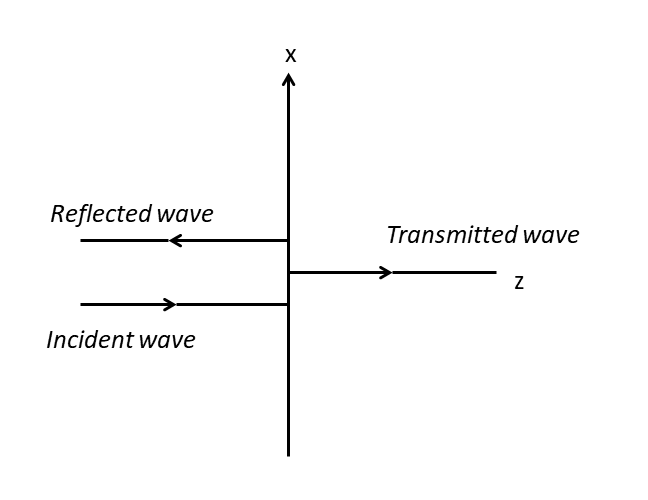
\includegraphics[scale=0.6]{./graphics/normal_incidence1}
\caption{Normal incidence at media interface}
\label{fig:16}
\end{figure}

So this case has essentially become like a one-dimensional propagation. The amplitude of the electric and magnetic fields now only varies in the z-direction. The fields thus correspond to a one-dimensional propagation in the z-direction. This is identical to the case of a transmission line where the waves travel along the transmission line and we are not bothered about the variation of the fields perpendicular to the transmission line.

At the interface, looking rightward beyond the boundary, we see an infinite medium ahead of intrinsic impedance $\eta_{2}$. looking from the interface to the left, we see another infinite medium with intrinsic impedance $\eta_{1}$. Thus, this case is similar to a scenario where we have two transmission lines of characteristic impedance $\eta_{1}$ and $\eta_{2}$. When the wave is incident from the left, it is like having a transmission line with characteristics impedance  $\eta_{1}$ terminated at a load impedance of  $\eta_{2}$ as shown in fig~\ref{fig:17}.
\begin{figure}[h]
\centering

\includegraphics[width=1\linewidth]{./graphics/17}
\caption{}
\label{fig:17}
\end{figure}

So we get $\Gamma_{\perp} = \frac{\eta_{2} - \eta_{1}}{\eta_{2} + \eta_{1}}$, the reflection coefficient of a line with characteristics impedance  $\eta_{1}$ and terminated at  $\eta_{2}$. Just like in the case of a transmission line of characteristics impedance $Z_{0}$ terminated at a load impedance $Z_{L}$ with a reflection coefficient $\Gamma = \frac{Z_{L} - Z_{0}}{Z_{L} + Z_{0}}$.

So the case of normal incidence which is a special case for any oblique incidence at a dielectric media interface is equivalent to the case of the transmission line. So when we were dealing with the transmission lines, we were essentially handling one of the special cases of reflections at the dielectric media interface. Also, we saw that when a transmission line was terminated in  $\eta_{2}$, the power was getting lost in  $\eta_{2}$ which was located at the load end. But now that we are having a media interface,  the power is not lost at that location(the interface) but rather goes into the second medium. So equivalently, we can say that this is like a transmission line but the power lost at the dielectric boundary is the same as the power lost into  $\eta_{2}$ as the terminating impedance of the transmission line. 

For this normal incidence case with $\theta_{i}$ = $\theta_{t}$ = 0, for parallel polarization,

\begin{dmath*}
\Gamma_{\parallel} = \frac{\eta_{1} cos\theta_{i} - \eta_{2} cos\theta_{t}}{\eta_{2} cos\theta_{t} + \eta_{1} cos\theta_{i}}
= \frac{\eta_{1} -\eta_{2}}{\eta_{2} +\eta_{1}}
\end{dmath*}
\begin{dmath*}
\tau_{\parallel} = \frac{2\eta_{2} cos\theta_{i} }{\eta_{2} cos\theta_{t} + \eta_{1} cos\theta_{i}} 
= \frac{2\eta_{2}}{\eta_{2} + \eta_{1}}
\end{dmath*}

$\Gamma_{\perp}$ and $\Gamma_{\parallel}$ having opposite signs is due to the fact that for  $\Gamma_{\perp}$, $E_{i}$ and $E_{r}$ had same direction. However, for  $\Gamma_{\parallel}$, $E_{i}$ and $E_{r}$ had opposite directions in the tangential components of the electric field that was used to solve for the boundary condition. So the reflection coefficient in the case of normal incidence is generally written as $\Gamma = \frac{\eta_{2} - \eta_{1}}{\eta_{2} + \eta_{1}}$  with the assumption that the electric fields are oriented in the same direction. If $\eta_{1}>\eta_{2}$ we have a phase reversal of the reflected wave and if $\eta_{2}>\eta_{1}$, there will be no phase reversal. 

So irrespective of the medium parameters and angle of incidence, the reflection and transmission coefficient are all real quantities. There may be direction reversal for the electric and magnetic fields,  but there is no arbitrary phase change either in the transmitted or reflected wave. This case is a rather simple reflection and refraction case. Later, we will consider a special case where there is a possibility of having a phase change not $0$ or $\pi$ in the transmitted and reflected waves.
